\subsection{Разведочные абляции}
Разведочный этап служит только для выбора гипотезы; его улучшения не являются подтверждением на новых данных.
В таблице --- отношения средних EDR к baseline. Значение меньше единицы означает меньшую ошибку.
\begin{center}\small\setlength{\tabcolsep}{4pt}
\begin{tabular}{@{}lrrrrrr@{}}\toprule
 & \multicolumn{3}{c}{additive} & \multicolumn{3}{c}{quadratic}\\
Вариант & $m=2$ & $m=3$ & $m=5$ & $m=2$ & $m=3$ & $m=5$\\\midrule
gls & 0.877 & 1.054 & 0.956 & 0.790 & 0.800 & 0.710\\
row & 0.969 & 1.035 & 0.985 & 0.856 & 0.820 & 0.759\\
neff & 1.007 & 1.100 & 0.992 & 1.012 & 0.983 & 1.134\\
floor0.01 & 1.000 & 1.000 & 1.000 & 1.000 & 1.000 & 1.000\\
floor0.05 & 1.000 & 1.027 & 0.972 & 1.000 & 0.973 & 1.000\\
floor0.1 & 1.000 & 1.029 & 0.972 & 1.000 & 0.984 & 1.000\\
floor0.2 & 1.000 & 1.019 & 0.950 & 1.000 & 0.967 & 1.000\\
gls-floor0.01 & 0.877 & 0.995 & 0.958 & 0.790 & 0.800 & 0.710\\
gls-floor0.05 & 0.877 & 1.076 & 0.998 & 0.790 & 0.800 & 0.710\\
gls-floor0.1 & 0.877 & 1.092 & 0.963 & 0.790 & 0.800 & 0.710\\
gls-floor0.2 & 0.866 & 1.066 & 0.962 & 0.790 & 0.799 & 0.710\\
\bottomrule\end{tabular}\end{center}
Выбран кандидат \code{gls-floor0.01}; после выбора его настройки зафиксированы.
\subsection{Проверка выбранного кандидата на новых seed}
\textbf{selection: допуск не пройден.} 
Кластерный $95\%$ интервал среднего парного изменения EDR на additive $m=3,5$: $[-0.01733, 0.03669]$.
\begin{center}\small\setlength{\tabcolsep}{5pt}
\begin{tabular}{@{}lrrrrrr@{}}\toprule
Функция & $m$ & Начало & Baseline & Кандидат & Отношение & Победы\\\midrule
additive & 2 & 0.2448 & 0.0599 & 0.0533 & 0.890 & 8/10\\
additive & 3 & 0.5660 & 0.4811 & 0.4934 & 1.026 & 4/10\\
additive & 5 & 0.7133 & 0.6456 & 0.6496 & 1.006 & 5/10\\
quadratic & 2 & 0.2630 & 0.0649 & 0.0486 & 0.748 & 9/10\\
quadratic & 3 & 0.3683 & 0.0855 & 0.0557 & 0.651 & 10/10\\
quadratic & 5 & 0.3247 & 0.1158 & 0.0848 & 0.732 & 8/10\\
\bottomrule\end{tabular}\end{center}
Условия допуска: полные пары --- да; ортогональность --- да; снижение ошибки на основных случаях --- нет; отрицательный доверительный интервал --- нет; допустимая ошибка на остальных случаях --- да.
\textbf{Validation не запускалась}: заранее установленные условия selection не выполнены. Повторная настройка по этому этапу не проводилась.
\begin{center}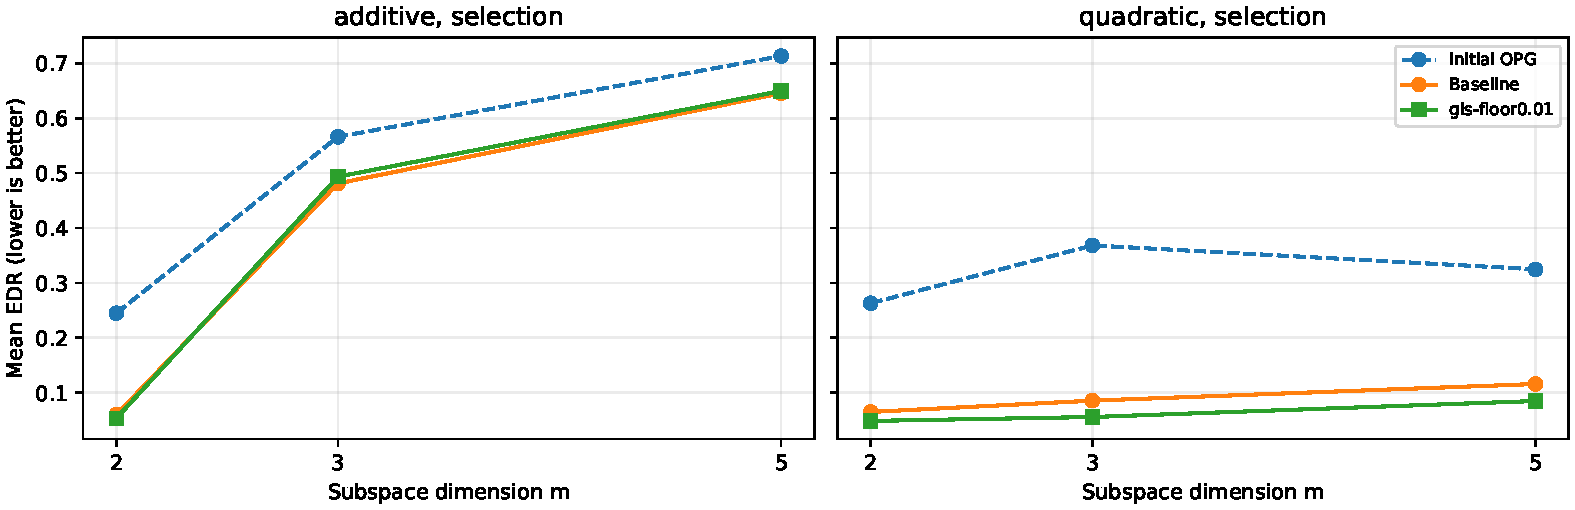
\includegraphics[width=\linewidth]{edr_metric_results_plot.pdf}\end{center}
\subsection{Время, память и диагностический сертификат}
\begin{center}\small\begin{tabular}{@{}lrr@{}}\toprule Величина & Baseline & Кандидат\\\midrule
Медиана fit time, с & 1.262 & 1.568\\
Медиана полного времени процесса, с & 1.651 & 1.896\\
Медиана peak RSS до диагностики, МиБ & 130.232 & 130.688\\
\bottomrule\end{tabular}\end{center}
Полное время включает запуск Python, загрузку данных и, у baseline, отдельную диагностическую процедуру (медиана 0.059 с). В fit time она не включена. Замеры выполнены при трёх конкурирующих процессах, BLAS по одному потоку; это не последовательный микробенчмарк.
\begin{center}\small\begin{tabular}{@{}lrr@{}}\toprule Диагностика внутренних вызовов & Baseline & Кандидат\\\midrule
Всего вызовов & 300 & 300\\
Сходимость по внутреннему критерию & 0 & 0\\
Остановка по max\_steps & 261 & 231\\
Вызовы с потерей локального ранга & 300 & 300\\
Применим гладкий критерий стационарности & 0 & 0\\
\bottomrule\end{tabular}\end{center}
Завершение fit без исключения означает получение конечного ортонормированного базиса, но не доказывает сходимость внутренних задач или достижение глобального минимума. Цели разных метрик имеют разный масштаб и по их значениям качество восстановления не сравнивается.
В 60/60 baseline-fit предварительная процедура встретила вырожденную $C_j$: условие теоремы $C_j\succ0$ не выполнено. Это возможно даже при средней массе 50: некоторые периферийные центры имеют слишком мало соседей. Ridge-инициализация остаётся определённой, но формулу для нерегуляризованных градиентов к ней применять нельзя. Сертифицированное принятие шага в таких fit не выполнялось.
Число центр--итераций с регуляризацией положительного спектра: 16043; с полностью нулевой ковариацией у кандидата: 1721. Нулевые информационные блоки дают нулевую невязку и сохраняются в трассе.
Аудит основного исследования: 336/336 успешных fit, геометрические ошибки и контрольные суммы сохранённых данных проверены повторно.
\subsection{Сохранённая первая попытка}
В \code{attempt1-zero-covariance} сохранён первоначальный запуск. Первый прототип ошибочно отклонял все нулевые ковариационные блоки; случай окна с единственным наблюдением воспроизведён отдельным тестом и исправлен. После исправления использованы новые диапазоны seed. Неудачи первой попытки не заменены успешными строками.
В первой попытке кандидат floor0.05 также не прошёл selection: $m=3$, отношение средних EDR 1.0349; $m=5$, отношение средних EDR 0.9931. Этот отрицательный результат сохраняет силу для той попытки.
\subsection{Вывод по эксперименту}
Выбранная поправка не прошла все заранее заданные условия. Локальные улучшения следует считать ограниченным эмпирическим эффектом; оснований менять стандартный алгоритм по этому эксперименту нет.
